\section{Results and Discussion}

This section discusses the findings of the experiments, analyzing the strengths and weaknesses of the proposed models. The analysis focuses on the following aspects:

\begin{itemize}
    \item \textbf{Effectiveness and comparison of the models:} Each model's performance at different frequencies and the reasons for their effectiveness.
    
    \item \textbf{Limitations of the approach:} Potential limitations of each model.
    
    \item \textbf{Future work:} Future directions that could be explored to improve the performance of the models.
\end{itemize}

\subsection{Effectiveness and Comparison of the Models}

Initially, we focused on predicting daily average DC power using both univariate (only lagged DC power) and multivariate (including lagged ambient temperature, module temperature, and irradiation) setups.

\begin{figure}[h]
    \centering
    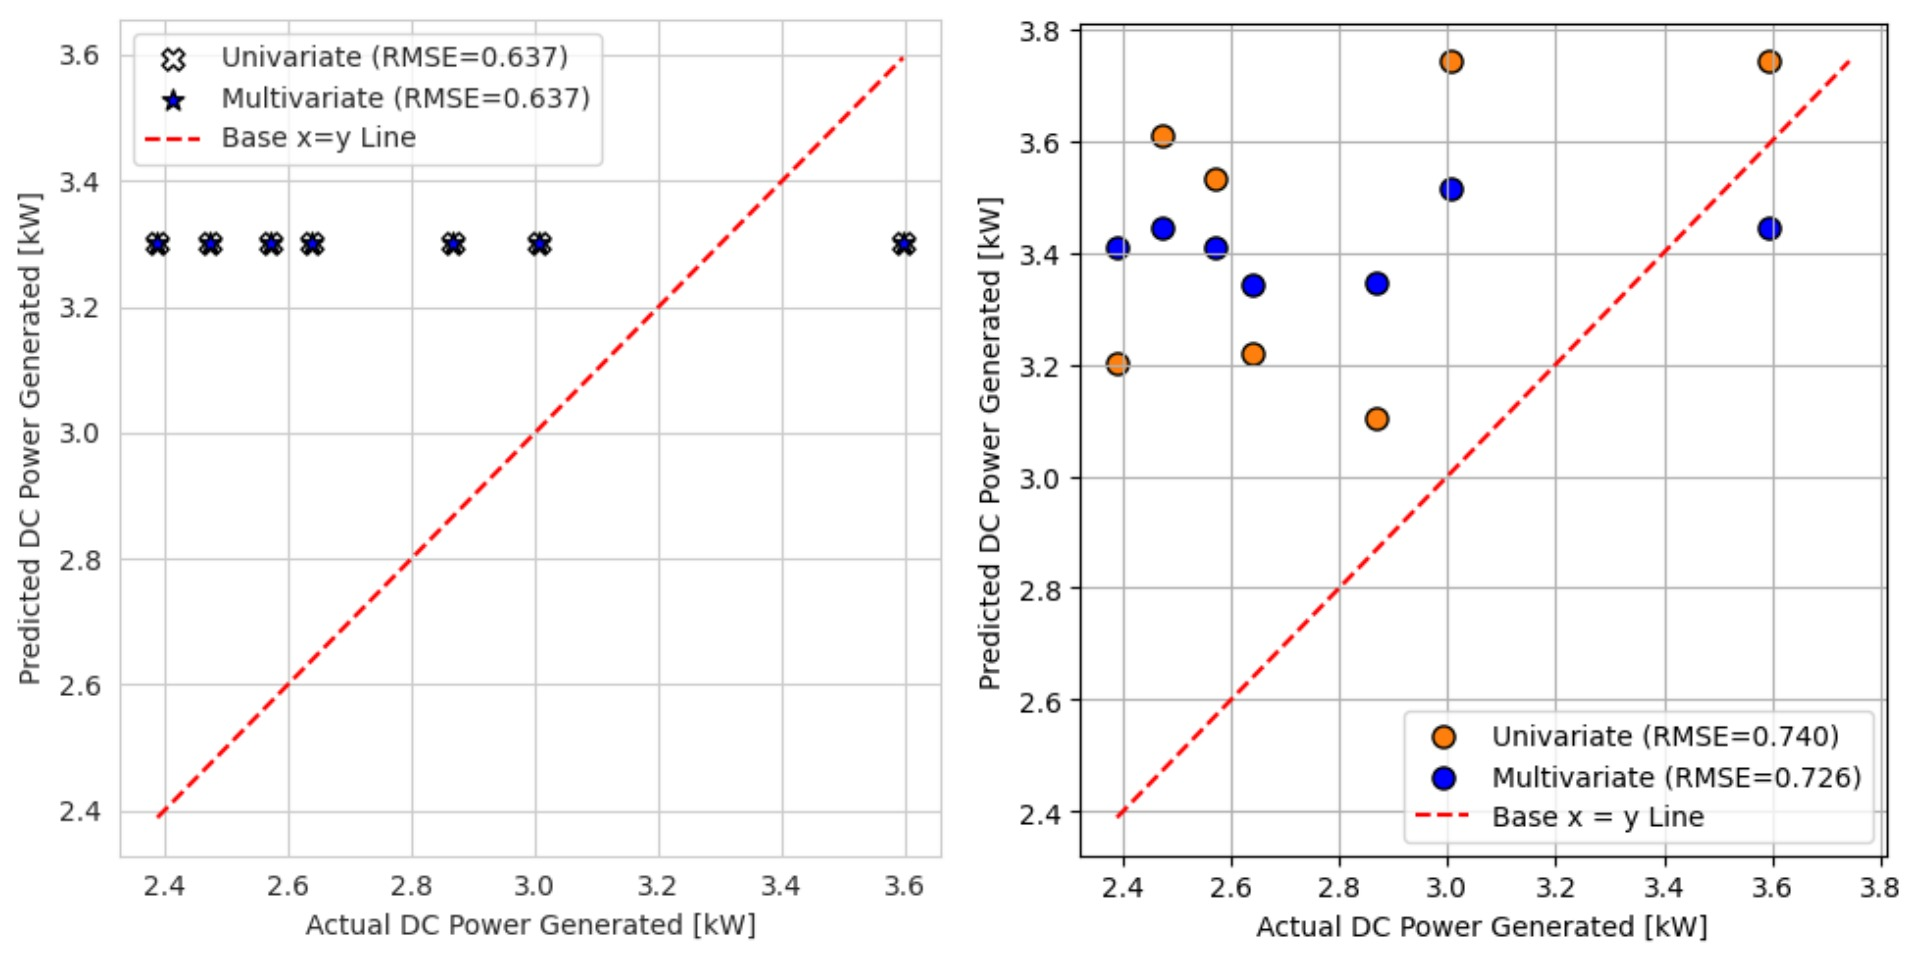
\includegraphics[width=0.5\textwidth]{Figures/uni-multi.jpg}
    \caption{Univariate with only DC Power and Multivariate: Actual vs Predicted for Lasso (left) and kNN (right)}
    \label{fig:uni-multi}
\end{figure}

As shown in Figure \ref{fig:uni-multi}, for the daily prediction frequency, the Lasso model with feature sets (D) and (D, A, I, M) both achieved an RMSE of 0.637. The kNN model performed slightly worse, with RMSE values of 0.740 for feature set (D) and 0.726 for feature set (D, A, I, M). This indicates that for daily predictions, the Lasso model is more effective. It's important to note that in both univariate and multivariate settings, the Lasso model, which utilized the default alpha (\(\lambda\)) value of 1.0, exhibited a particular behavior. When alpha is set to 1.0, the regularization penalty is high, leading to the coefficient for DC power being shrunk to zero for the univariate model and all the other features including DC power in the multivariate model. This effectively nullifies the influence of these features on the prediction. In such a scenario, the Lasso model relies solely on the intercept term to make predictions. Consequently, regardless of the input, the model will always predict the average DC power observed during training.
This behavior explains the consistent RMSE value of 0.637 for Lasso in both the univariate and multivariate daily predictions. While Lasso technically outperforms kNN in these cases, its predictive power is limited by the high regularization strength, rendering it equivalent to a simple average predictor. However, the high RMSE values for both models highlight the lack of precision we encountered. Therefore, we transitioned to hourly training data to aim for an RMSE of 0.5 or lower, and perform hyperparamter tuning to achieve better regularization.

On an hourly basis, we examined which features were most relevant and how well each algorithm could capture the trend. It was found that Irradiation and DC power were the most informative features, likely due to their high correlation, as depicted in Figure \ref{fig:hourDC}.

\begin{figure}[h]
    \centering
    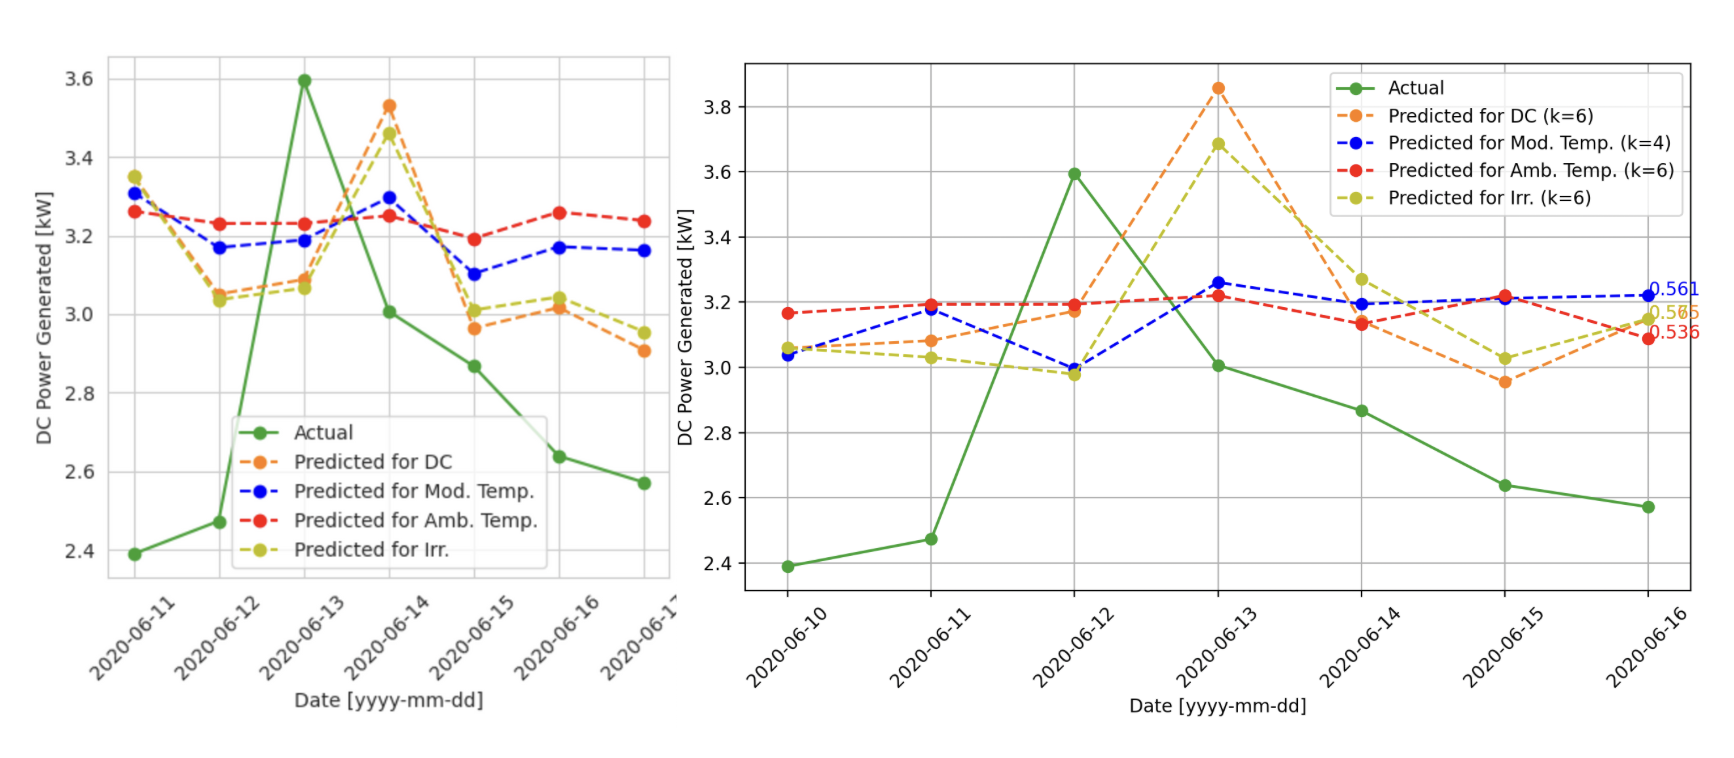
\includegraphics[width=0.5\textwidth]{Figures/hourDC.png}
    \caption{Trends for univariate prediction with time series cross-validation on an hourly training basis: Lasso (left) and kNN (right)}
    \label{fig:hourDC}
\end{figure}

However, even with time series cross-validation and hyperparameter tuning in multivariate settings with DC power as a reference feature, we were unable to improve the models' ability to capture the intra-day variations in DC power. This is illustrated in Figure \ref{fig:hourDCF}.

\begin{figure}[h]
    \centering
    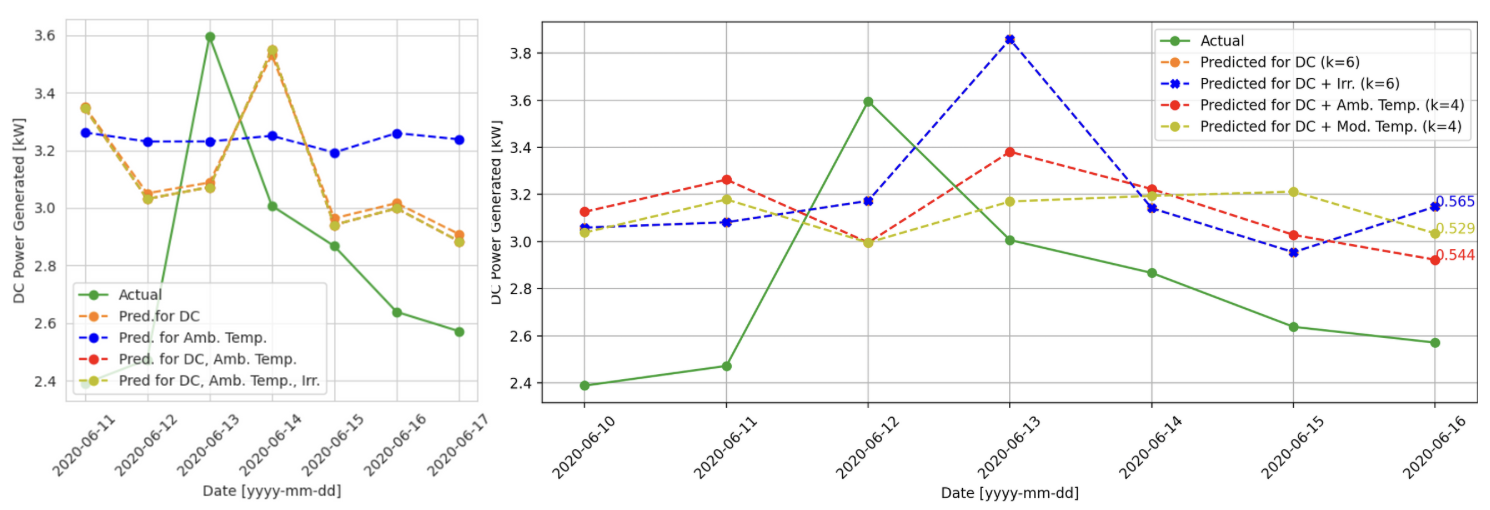
\includegraphics[width=0.5\textwidth]{Figures/hourDCF.png}
    \caption{Trends for multivariate with feature set combinations: Lasso (left) and kNN (right)}
    \label{fig:hourDCF}
\end{figure}

\begin{figure}[h]
    \centering
    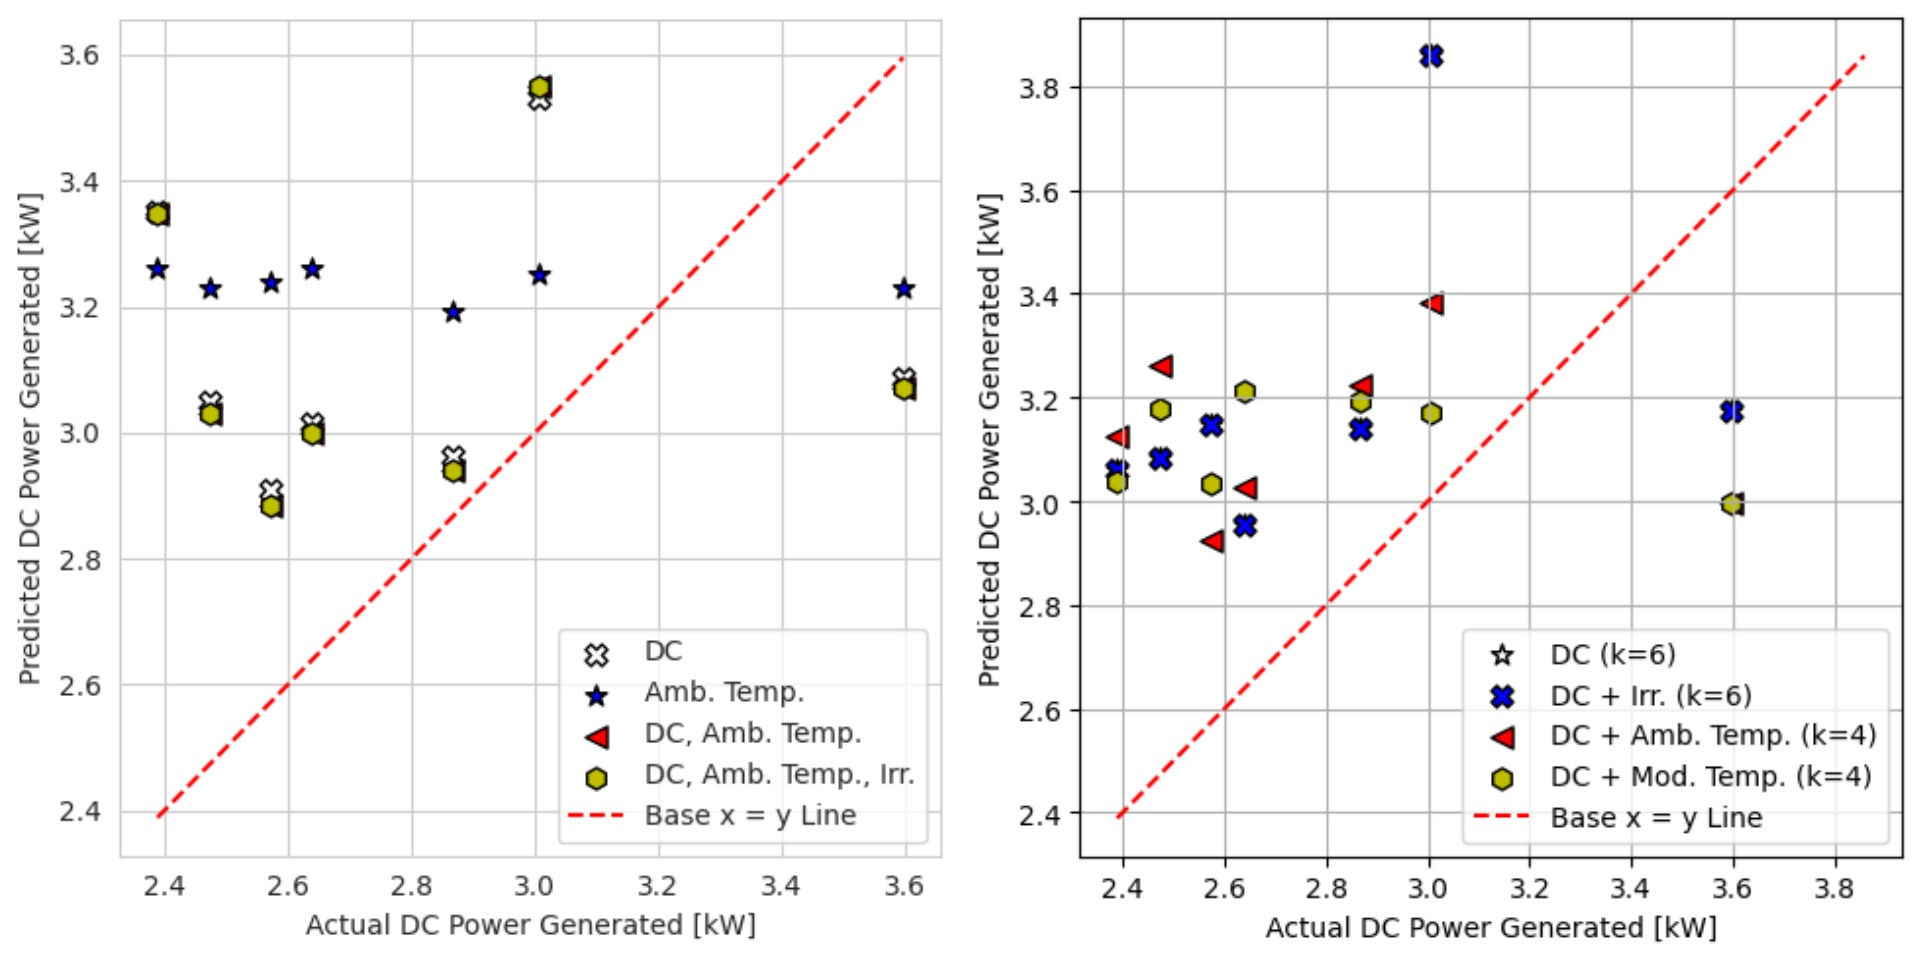
\includegraphics[width=0.5\textwidth]{Figures/multi_pred_vs_actual.jpg}
    \caption{Multivariate with feature set combinations: Actual vs Predicted for Lasso (left) and kNN (right)}
    \label{fig:multi-pred-actual}
\end{figure}

As shown in Figure \ref{fig:multi-pred-actual}, both models tend to overpredict on average, which suggests a potential area for future improvement.

\begin{table}[h]
    \centering
    \caption{Lasso coefficient selection with feature combinations}
    \begin{tabular}{|l|l|l|l|l|l|l|} 
    \hline
    $\beta_h$ & $h=1$ & $h=2$ & $h=3$ & $h=4$ & $h=5$ & $h=6$ \\ 
    \hline
    $D$ & 0 & 0 & 0 & 0 & 0 & 0 \\ 
    \hline
    $A$ & 0 & 0 & 0 & 0 & 0 & 0 \\ 
    \hline
    $D,A$ & 0,0 & 0,0 & 0,0 & 0,0 & 0,0 & 0,0 \\ 
    \hline
    $D,A,I$ & 0,0,0 & 0,0,0 & 0,0,0 & 0,0,0 & 0,0,0 & 0,0,0 \\ 
    \hline
    $\beta_h$ & $h=7$ & $h=8$ & $h=9$ & $h=10$ & $h=11$ & $h=12$ \\ 
    \hline
    $D$ & 0 & 0 & 0 & 0 & 0 & \textbf{0.04} \\ 
    \hline
    $A$ & 0 & 0 & 0 & 0 & 0 & 0 \\ 
    \hline
    $D,A$ & 0,0 & 0,0 & 0,0 & 0,0 & 0,0 & \textbf{0.04},0 \\ 
    \hline
    $D,A,I$ & 0,0,0 & 0,0,0 & 0,0,0 & 0,0,0 & 0,0,0 & \textbf{0.04},0,0 \\ 
    \hline
    $\beta_h$ & $h=13$ & $h=14$ & $h=15$ & $h=16$ & $h=17$ & $h=18$ \\ 
    \hline
    $D$ & \textbf{0.08} & 0 & 0 & 0 & 0 & 0 \\ 
    \hline
    $A$ & \textbf{0.01} & 0 & 0 & 0 & 0 & 0 \\ 
    \hline
    $D,A$ & \textbf{0.08},0 & 0,0 & 0,0 & 0,0 & 0,0 & 0,0 \\ 
    \hline
    $D,A,I$ & \textbf{0.08},0,0 & 0,0,0 & 0,0,0 & 0,0,0 & 0,0,0 & 0,0,0 \\ 
    \hline
    $\beta_h$ & $h=19$ & $h=20$ & $h=21$ & $h=22$ & $h=23$ & $h=24$ \\ 
    \hline
    $D$ & 0 & 0 & 0 & 0 & 0 & 0 \\ 
    \hline
    $A$ & \textbf{0.02} & 0 & 0 & 0 & 0 & 0 \\ 
    \hline
    $D,A$ & 0,0 & 0,0 & 0,0 & 0,0 & 0,0 & 0,0 \\ 
    \hline
    $D,A,I$ & 0,0,0 & 0,0,0 & 0,0,0 & 0,0,0 & 0,0,0 & 0,0,0 \\ 
    \hline
    \end{tabular}
    \label{tab:coeff_lasso}
\end{table}

A detailed examination of the Lasso coefficient table (Table \ref{tab:coeff_lasso}) indicates that most coefficients, even during peak power generation hours (6 AM to 6 PM), are zero. This sparsity highlights Lasso's tendency to select only the most critical features, effectively ignoring others. Notably, specific hours such as hour 13 are used by Lasso, reinforcing the model's focus on particular time slots for prediction. Furthermore, analysis of the alpha vs. RMSE graph (Figure \ref{fig:rmse-vs-alpha}) demonstrates that adding more than two feature combinations results in similar outcomes, effectively removing those additional features from being used in training. This behavior underscores the importance of feature selection in optimizing model performance without overfitting.

\subsection{Limitations of the Approach}

The primary limitation we encountered stemmed from the dataset itself. The high volatility inherent in daily power output, combined with the relatively small sample size (34 days), likely hindered the models' ability to discern clear patterns.

This issue also affected the cross-validation step, as the small number of points in the test set (only 7) restricted the applicability of kNN for a higher number of neighbors, as shown in Figure \ref{fig:CV_F_Evo}.

\begin{figure}[h]
    \centering
    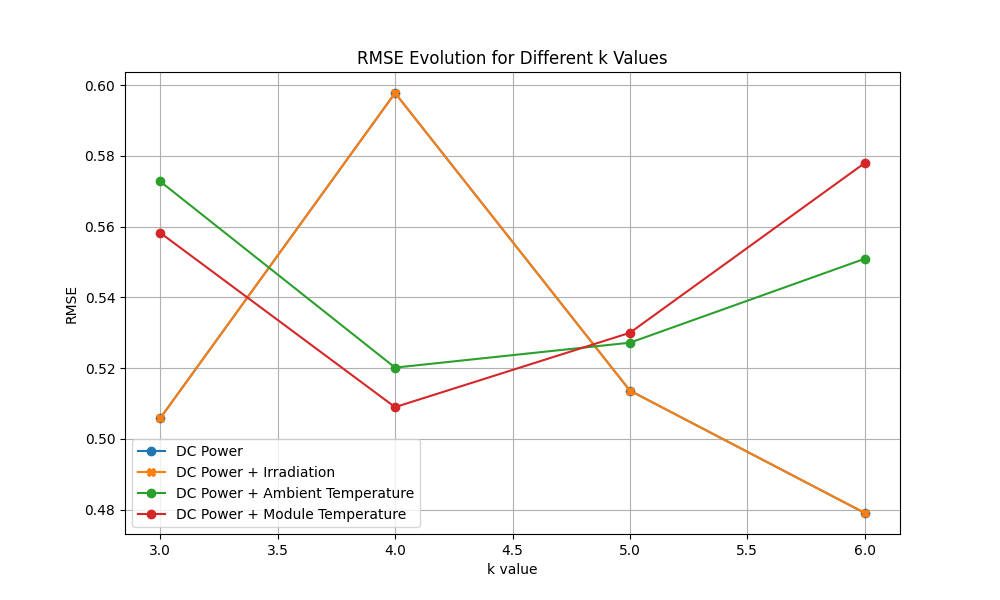
\includegraphics[width=0.5\textwidth]{Figures/CV_F_Evo.png}
    \caption{Evolution of RMSE as a function of the number of neighbors $k$ in the kNN algorithm for multivariate with feature set combinations}
    \label{fig:CV_F_Evo}
\end{figure}

Increasing the test set size to ten points confirmed this theory, allowing kNN to achieve an RMSE of 0.49 using DC power and module temperature as combined features.

It may be noticed that Lasso algorithm seemed to not be sensitive to this issue.

\begin{figure}[h]
    \centering
    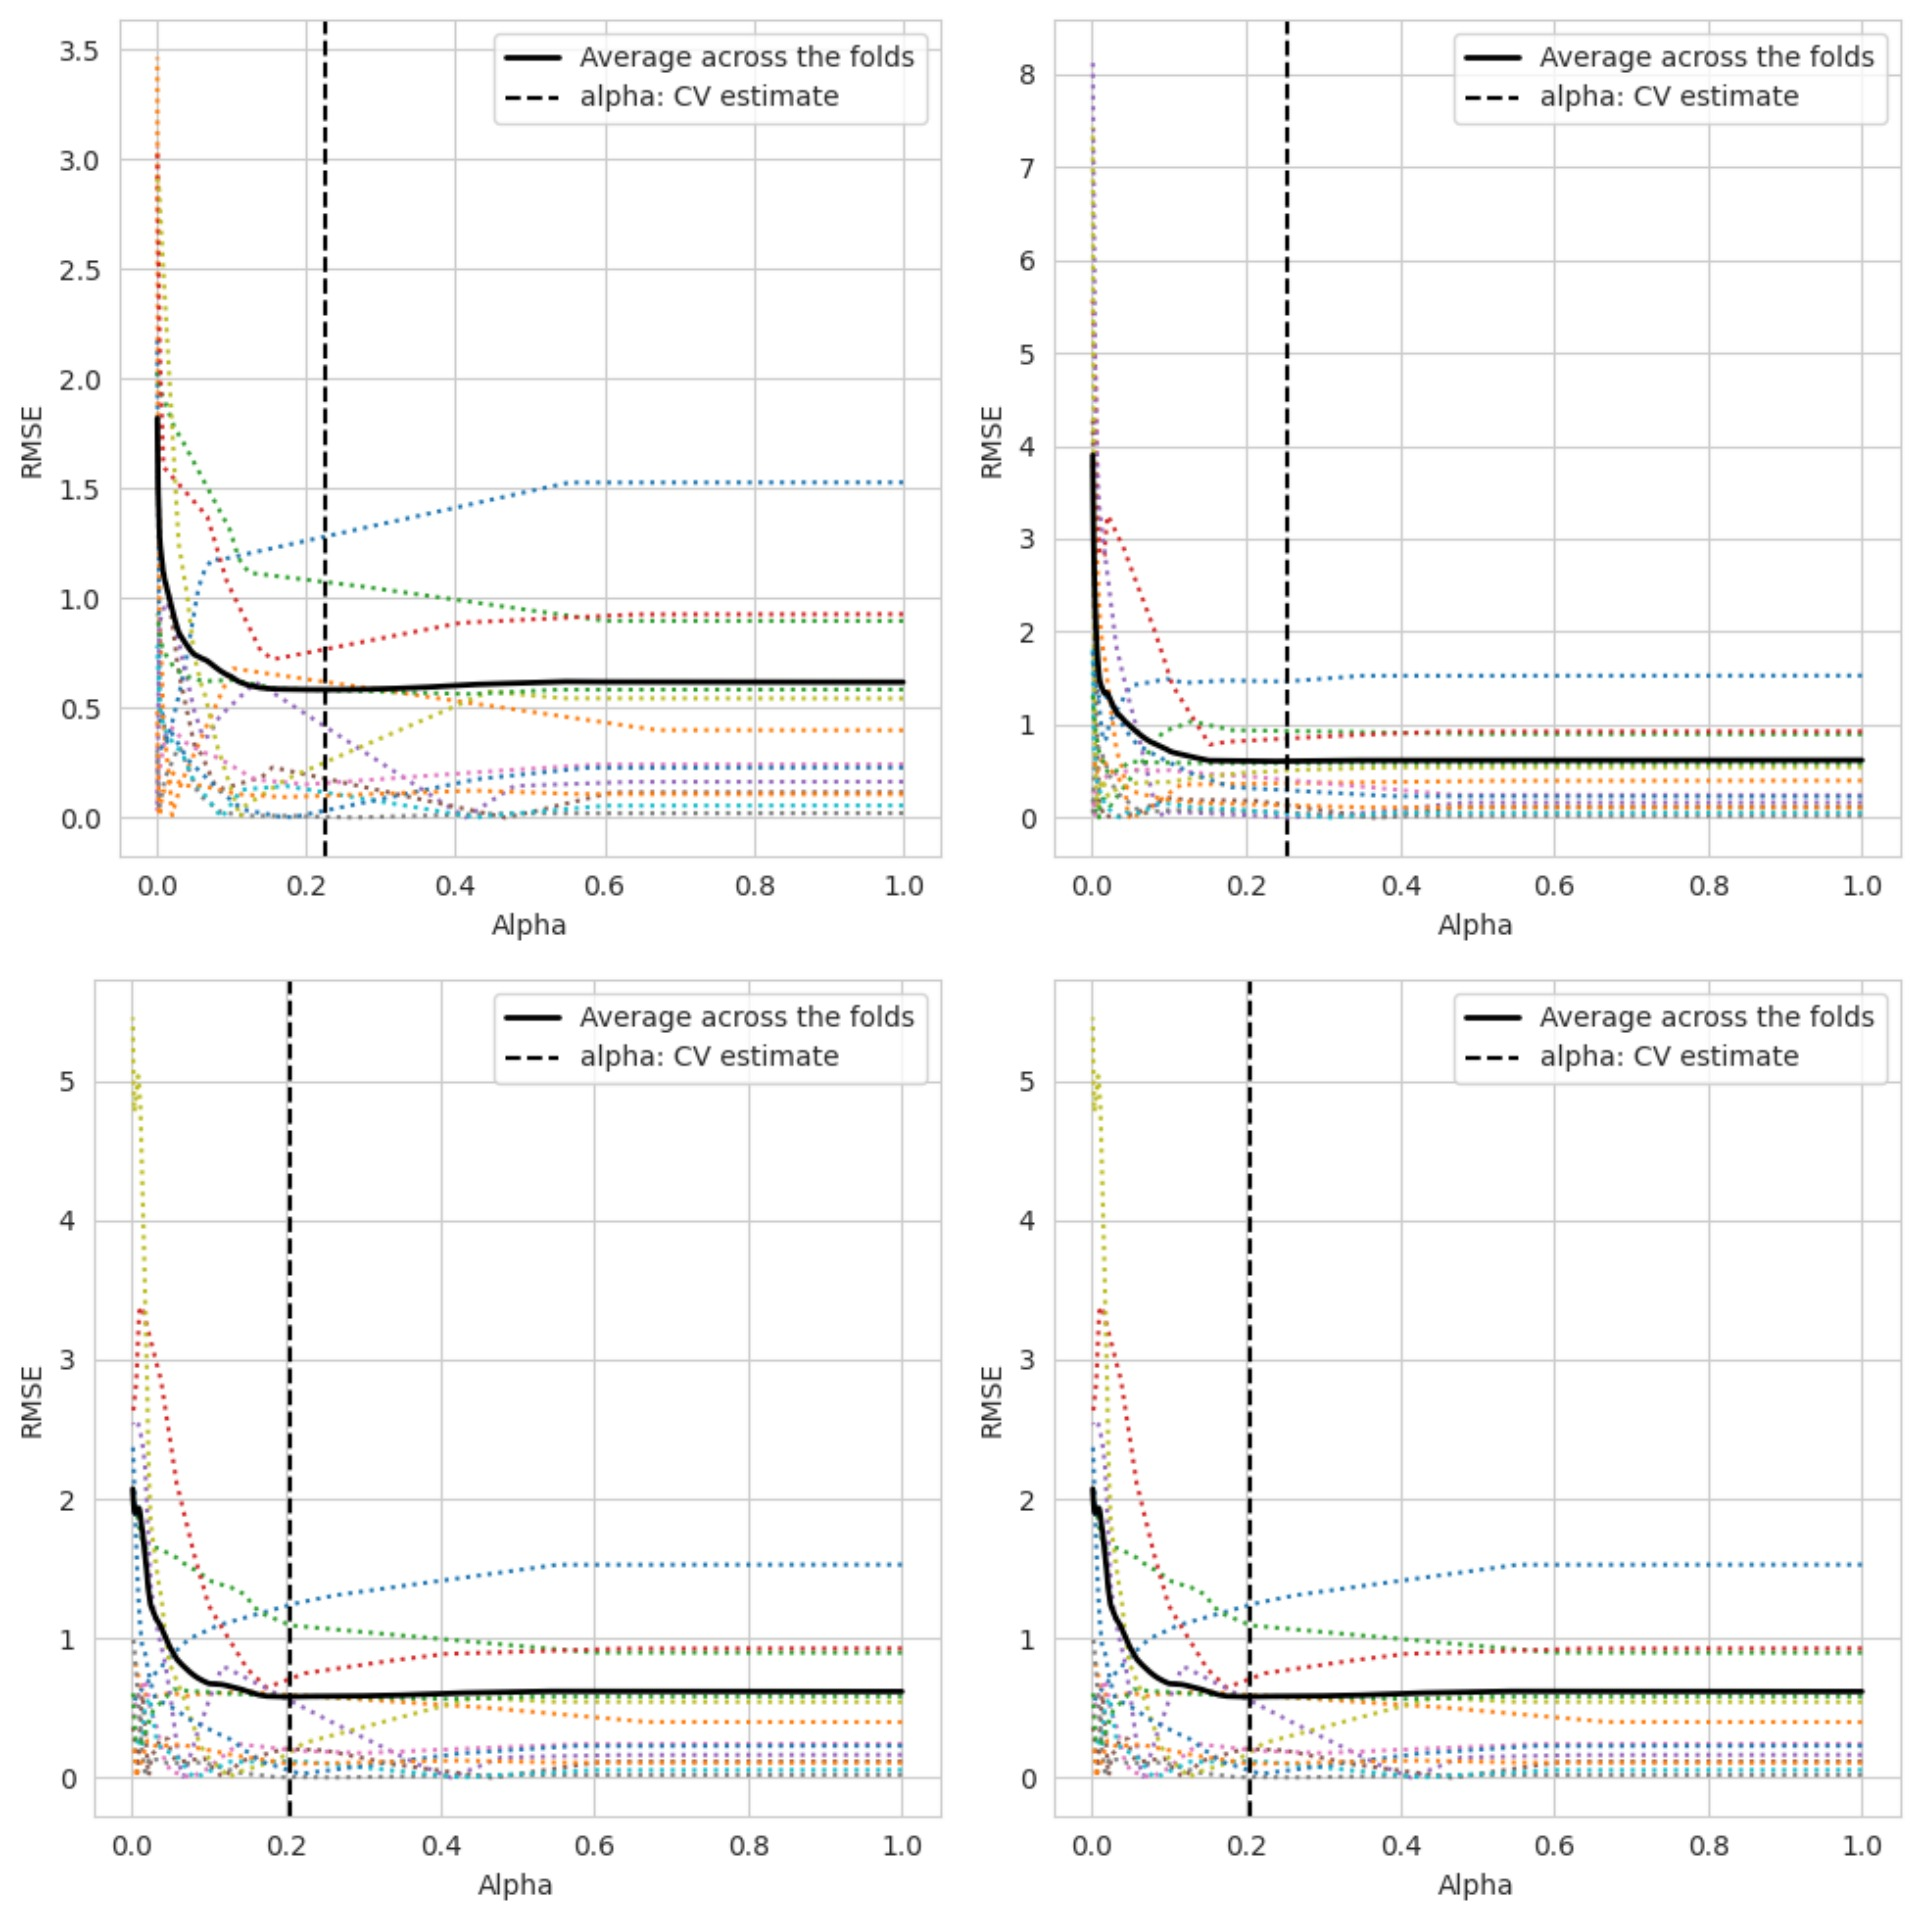
\includegraphics[width=0.5\textwidth]{Figures/rmse_vs_alpha_lasso.jpg}
    \caption{RMSE vs. regularization strength ($\lambda$) for Lasso models with varying feature sets}
    \label{fig:rmse-vs-alpha}
\end{figure}

\subsection{Future Work}

Future research could explore the following directions:

\begin{itemize}
    \item \textbf{Data processing:} Increase the dataset length or use a different dataset with more samples to improve the models' ability to capture trends and reduce the impact of volatility. A larger and more diverse dataset could enhance the robustness of the predictions.
    \item \textbf{Advanced Modeling Techniques:} Explore and implement advanced machine learning algorithms such as Random Forest, Gradient Boosting Machines, or Deep Learning models. These methods may provide better performance by capturing complex patterns in the data.
    \item \textbf{Feature Engineering:} Investigate additional features that could improve prediction accuracy, such as incorporating weather forecasts, historical power generation data, and real-time sensor data.
    \item \textbf{Optimization Techniques:} Further fine-tune hyperparameters using advanced optimization methods like Bayesian Optimization.
\end{itemize}

\begin{table}[h]
    \centering
    \caption{Model Performance for Predicting Current Day Average DC Power}
    \begin{tabular}{|l|l|l|r|r|r|} 
    \hline
    \textbf{Model} & \textbf{Frequency} & \textbf{Features} & \textbf{$k$} & \textbf{$\lambda$} & \textbf{RMSE} \\ \hline
    Lasso & Day & D & - & 1.0 & 0.637 \\ \hline
    Lasso & Day & D, A, I, M & - & 1.0 & 0.637 \\ \hline
    LassoCV & Hour & D & - & 0.225 & 0.542 \\ \hline
    LassoCV & Hour & A & - & 0.253 & 0.593 \\ \hline
    \textbf{LassoCV} & \textbf{Hour} & \textbf{D, A} & - & \textbf{0.206} & \textbf{0.538} \\ \hline
    LassoCV & Hour & D, A, I & - & 0.206 & 0.538 \\ \hline
    kNN & Day & D & 7 & - & 0.740 \\ \hline
    kNN & Day & D, A, I, M & 7 & - & 0.726 \\ \hline
    kNN CV & Hour & D & 6 & - & 0.565 \\ \hline
    kNN CV & Hour & A & 6 & - & 0.536 \\ \hline
    kNN CV & Hour & I & 4 & - & 0.570 \\ \hline
    kNN CV & Hour & M & 6 & - & 0.561 \\ \hline
    kNN CV & Hour & D & 6 & - & 0.565 \\ \hline
    kNN CV & Hour & D, A & 4 & - & 0.544 \\ \hline
    \textbf{kNN CV} & \textbf{Hour} & \textbf{D, M} & \textbf{4} & - & \textbf{0.529} \\ \hline
    \end{tabular}
    \label{tab:model_comparison}
\end{table}